\documentclass[11pt,twoside]{report}
\usepackage{preamble}
\graphicspath{{../img/ch3/}}
\setcounter{chapter}{2}



\begin{document}

\chapter{Observing Zebrafish in 2D}
\label{chapter:fish_2d}




In this chapter we will focus on the methodology to observe zebrafish, swimming in a quasi two dimensional environment. The system was chosen for technical conveniences, as the 2D movement of fish can be captured by a digital camera easily. In comparison, recording the 3D movement of fish is a harder task, which will be discussed in chapter~\ref{chapter:fish_3d}. %and appendix~\ref{chapter:multi_view}.


\section{Introduction}


The majority of the studies on the collective behaviour of fish were performed in a quasi-2D environment, where the fish were confined in a shallow water tank \cite{miller2007, strandburg-peshkin2013, heras2019, sridhar2021}. The collective motion of the fish can be captured by digital cameras and process by image processing algorithms, generating the trajectories for all fish individuals.
%\marginfootnote{The zebrafish were usually recorded as grayscale videos, in contract to the coloured videos taken by conventional cameras. This is because the zebrafish are not colourful. Therefore, the different colour channels (red, green, blue) are often not very helpful for identifying the fish individuals in the video.}

The crucial step in this tracking process, is to correctly locate the fish, and identify their identities. A considerable amount of softwares have been designed to tackle the problem. For instance, \citeauthor{perez-escudero2014} published an algorithm that is capable of determining the identity of the fish from its image, and using the information to obtain correct trajectories \cite{perez-escudero2014}.
The key observation from \citeauthor{perez-escudero2014}, is that the joint probability distribution of pixel distance and pixel intensity of a fish is unique. Five years later in 2019, the same group published an update method, that utilised an artificial neural network to identify the individual fish \cite{romero-ferrero2019}.
Unlike most machine learning solutions to computer vision problems, the algorithm from \citeauthor{romero-ferrero2019} requires no human label, thanks to a very carefully constructed preprocess pipeline, which makes it stands out as the state of art method in the year of 2022 \cite{walter2021}.


In addition to the ideas and algorithms, the realistic development and deploy of an animal tracking software requires a lot of engineering work. For instance, it is important to have a suitable programming language to maximise the performance of the algorithm. An accessible graphical user interface (\gls{GUI}) and application programming interface (\gls{API}) are also crucial. In addition, the software should be easy to install on a new machine. Practically, large research groups will develop a versatile research software, like those from \citeauthor{walter2021} \cite{walter2021}.


In this chapter, We will present a new 2D tracking method, whose results are suitable for the calculation of 3D locations of the fish. The key feature of our algorithm is the ability to locate fish without relying on their morphological details (see Fig.~\ref{fig:fish-detail} for examples).
Our new method is necessary, because the fish can swim closer or further to the camera in the 3D experiment, casting different shapes on the camera.
Therefore, the identity of the fish can not be uniquely determined from their shapes in the image, causing the identity-based approach (\cite{perez-escudero2014, romero-ferrero2019, walter2021}) to have reduced validity. The problem is termed \emph{no-detail tracking}, as the details (the size, darkness, and shape) of a fish in the image is not a reliable source for its identification.

\marginpar{
\centering
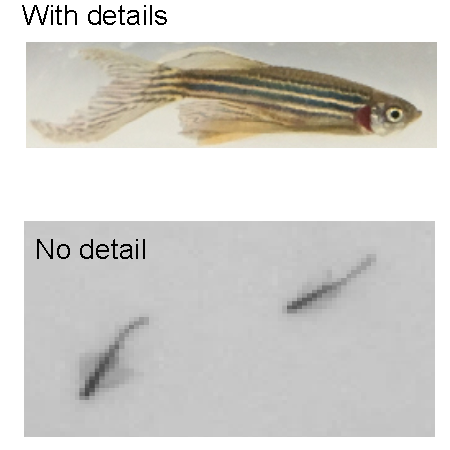
\includegraphics[width=\marginparwidth]{fish-detail}
\captionof{figure}[The morphological detail of a fish]{
	Top: a picture of zebrafish with various details. Bottom: a picture of two zebrafish with no detail.
}
\label{fig:fish-detail}
}

In the methods section, the ideas needed to carry out no-detail tracking will be discussed. The result of 2D swimming experiment, analysed by our method, will be presented in the results section. The 2D coordinates of zebrafish revealed two essential features. Firstly the spatial distribution of the fish was inhomogeneous. The effective pairwise interaction of the fish seemed attractive, and the attraction appear to decrease with the number of individuals in a group.

\section{Methods}

%Observing the fish in the lab includes the construction of the hardware, and the development of the software. Both of them will be covered in the method section. The 2D tracking code will be reused in chapter~\ref{chapter:fish_3d} as the basis for 3D tracking. 

\subsection{Fish and Apprautus}
\label{section:apprautus_2d}

The adult zebrafish, whose age is over one year old, were used to carry out the experiment. Most experiments in this section was carried out in the fish facility in Bristol, while some experiments were performed in room G59 in the HH Physics Laboratory in Bristol. The fish were fed three times a day, with natural day to night circles. The fish were hosted in their living tank before the experiments, with a density of 5 fish per litre of water. The water was filtered constantly, with a pH value close to 7 and the temperature close or above 25 °C.

Before each experiment, the fish were transferred from their living tank to the experimental environment, which will be referred to as the {\ot}. During the transfer, the fish were placed inside a temporary container, and then released into the {\ot}.
To make the fish stay in a quasi-2D environment, a flat plate was placed in a bowl-shaped tank, creating a shallow water environment (Fig.~\ref{fig:fish_apprautus_2d}). The shape of the bowl is especially chosen for a 3D tracking task, which will be introduced in chapter \ref{chapter:fish_3d}.



\begin{SCfigure}[][!ht]
  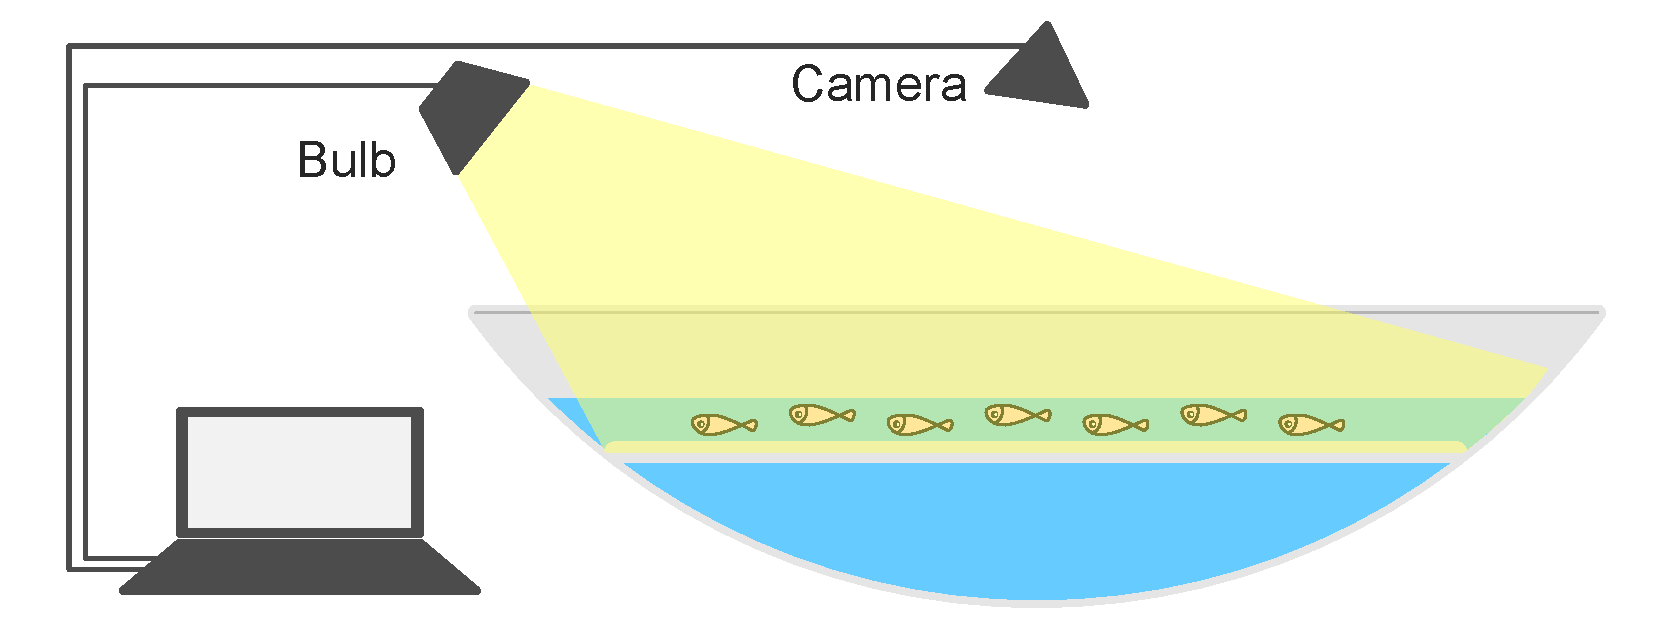
\includegraphics[width=\linewidth]{apprautus-2d}
  \caption[Two dimensional fish tracking apprautus]{\label{fig:fish_apprautus_2d}
  The apprautus to track the movement fish in a quasi-2D environment. The camera is placed above the fish to capture the top view. A computer controls the recording process as well as the illumination.
  }
\end{SCfigure}


\subsection{Metric Rectification}
\label{section:metric_rectify}


To record the video of the fish, a camera (Basler AC2040um) was fixed on top of the tank, as illustrated in Fig.~\ref{fig:fish_apprautus_2d}. The image size produced by our camera is 2056 pixels $\times$ 1540 pixels, at a frequency of 15 frames per second.
We mounted a 6 mm fixed focal length lens (C Series, Edmund Optics) on the camera, which yields a wide view, allowing us to place the camera closer to the fish group. The typical distance between the camera and the fish group is around 2 meters. With such setup, the fish (body length $\sim$ 30 mm) appear as black rods in the videos, as shown in Fig.~\ref{fig:metric-rectify}.


The image and videos obtained from the camera have three limitations, preventing it from being an accurate measurement tool.
The first issue is the distortion of images caused by the camera lens.
In addition, the cameras should be orientated exactly perpendicular to the water surface, so that the captured images were from the top view. Such accurate orientation is difficult to achieve without especially designed camera holders.
Finally, we also need to convert the unit of the image (pixels) to real life units (e.g. meters).
It is worth mentioning that these issues were more or less ignored in conventional 2D animal tracking tasks \cite{panadeiro2021}, and the present method is novel in the context of animal tracking.\marginfootnote{
Addressing these issues is ``less novel'' in the computer vision community focusing on the 3D reconstruction. It is impossible to retrieve 3D information correctly without understanding all the details about computers and photos.
}

To solve the problems, we need to \emph{calibrate} the camera, so that we know the distortion of the camera lens, the orientation of the camera, as well as the scale of objects in the images. To carry out the calibration, a chessboard (the calibration board) was placed on the surface of the water. And the image of the calibration board will offer enough information to tackle the aforementioned issues. 

The distortion can be recovered with standard camera calibration methods\marginfootnote{
The functions from the ``opencv'' library were used for the calibrations.
}
from the computer vision community \cite{ma2005, hartley2003}. The distortion is described with the following model,

$$
\begin{aligned}
x_{\text {distorted }} &= x\left(1+k_{1} r^{2}+k_{2} r^{4}+k_{3} r^{6}\right) \\
y_{\text {distorted }} &= y\left(1+k_{1} r^{2}+k_{2} r^{4}+k_{3} r^{6}\right)
\end{aligned}
$$

\noindent where $r$ is the radius of the pixels in the image with respect to the optical centre. And $k_i$ values are the distortion coefficients, which will be used to recover the undistorted image.


The imperfect orientation can be fixed by the knowledge of the camera as well. Briefly, the same 2D plane in the 3D space, will form different projections with different cameras. 
These different 2D projections are related to each other by a projective transformation.
Likewise, the same 2D plane for the fish in the imperfectly orientated camera is also related to its counterpart from a perfectly orientated camera.
Such a relation is termed as \emph{homography}
%\marginfootnote{Further description of the projective transformation, as well as the calculation of $\mathbf{H}$ is included in the appendix~\ref{chapter:multi_view}.}
, and can be represented by a matrix
$\mathbf{H} \in \mathbb{R}^{3 \times 3}$. This matrix can be calculated easily with the knowledge of the camera, following the method from \citeauthor{hartley2003} \cite{hartley2003}.
The homography allows us to transform the image from the imperfectly orientated camera, to a virtual image captured from a perfectly orientated camera. The transformed image is called the \emph{rectified image}.
From the rectified image, the scale can be recovered easily as we know the physical size of the calibration board. We call the rectified image with a known scale the \emph{metrically rectified image}.


Figure~\ref{fig:metric-rectify} shows an example of the metric rectification. Comparing the outline of boundary with/without distortion removed, it is clear that the raw image from the camera were distorted by the lens. The camera in the experiment were not perfectly perpendicular to the water surface, therefore the outline of the tank boundary appears to be an ellipse, because of the perspective transformation (\gls{homo}). The ellipse were reverted back to a circle (right subfigure, Fig.~\ref{fig:metric-rectify}) after the rectification process.

\begin{SCfigure}
  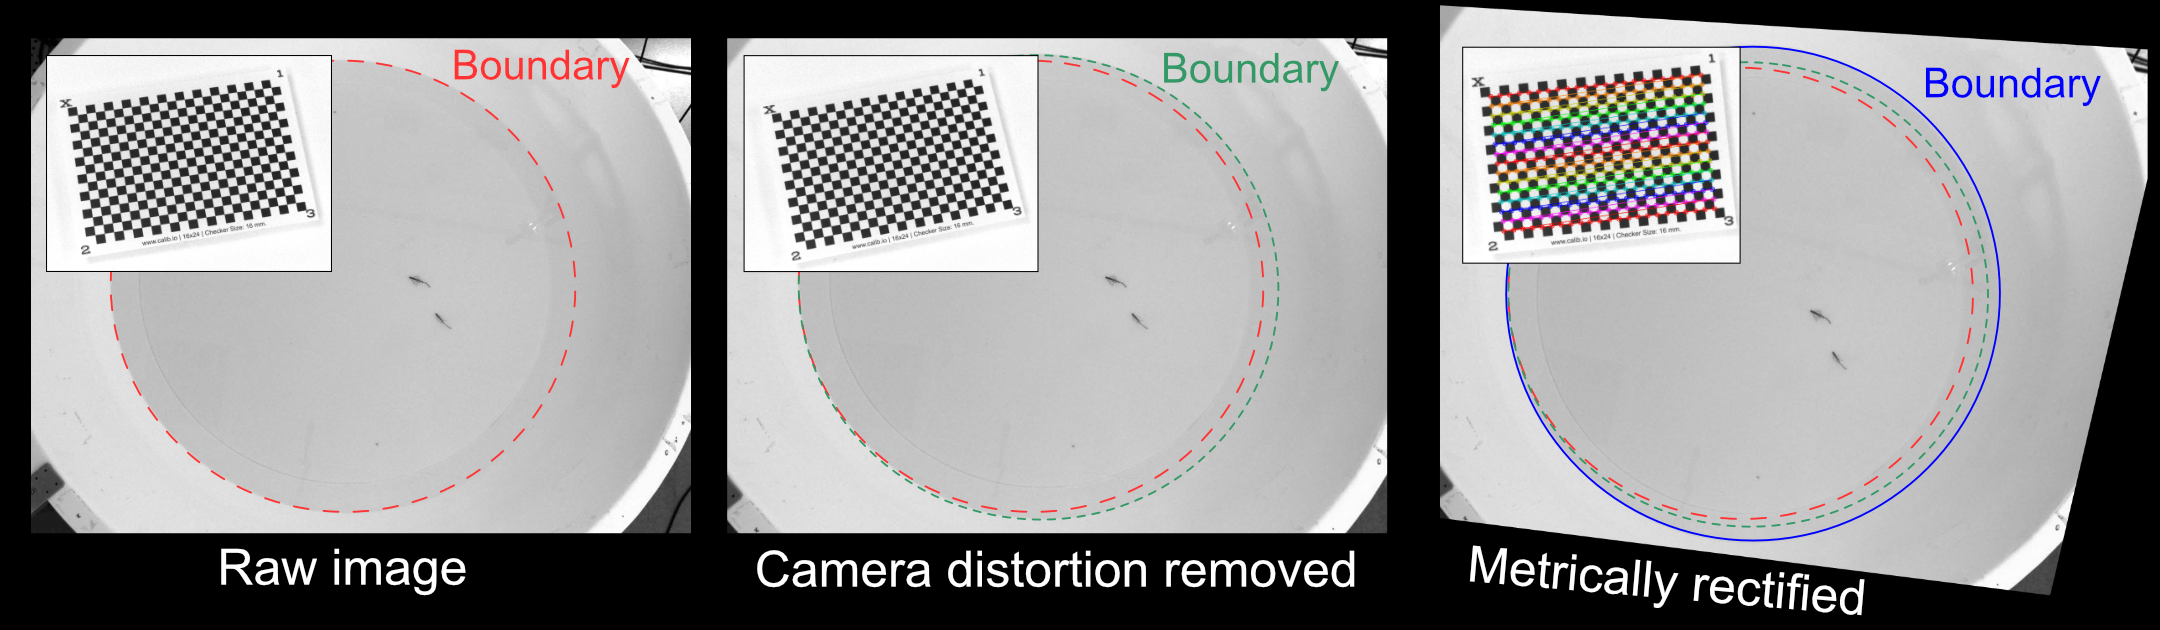
\includegraphics[width=\linewidth]{image-calib-2d.png}
  \caption[Metrical rectification of an image.]{
  	The process of metrical rectification. Left: the original image. Middle: the image where camera distortion being removed. Right: the metrically rectified image. The circular outline of the 2D boundary were outlined and overlaid, to stress the change of the image in different steps. The inserts in the figures correspond to the calibration pattern in each process.
  }
  \label{fig:metric-rectify}
\end{SCfigure}


Notably, the image rectification only ``works'' for the plane, where the calibration chessboard lies. For the fish data, the rectification is only accurate for the fish exactly swimming on the water-air interface. In other works, there will be tiny errors for the fish locations, when they swim inside the water. Such inaccuracy is fundamental for 2D fish tracking, since the fish is swimming a 3D space. To eliminate such error, we can carry out real 3D measurements, which will be introduced in chapter~\ref{chapter:fish_3d}.


\subsection{Image Processing}
\label{section:image_process}


The metrically rectified images of the fish contain the information about their behaviour.
To get useful information out of the image, we still need to perform image processing, to extract the coordinates of the fish from the images.

In a normal image, the fish appear as a dark spot (see Fig.~\ref{fig:metric-rectify} and Fig.~\ref{fig:2d_process} for instances).
Ideally, we want to work with images containing a collection of delta functions (see middle subplot of Fig.~\ref{fig:locate-cnn} for instance), where the pixel intensities in the centres of each individual fish is maximised, and the pixel intensities are zero everywhere else. Extracting the coordinates of fish from such image, will therefore be a trivial task, as we only need to find the pixels with non-zero values. Even though it is possible to construct such transformation directly with machine learning based approaches \cite{newby2018}, it is still not an easy task, without large amount of human labelled training data. Therefore, we restrict our goal for the image processing process to be the removal of the static background. As a result, the processed image should only contain the fish.

Traditional image processing methods, such as thresholding, blurring, and morphological operations, were used in this project to perform the background removal task.
As a result, we get a \emph{foreground video} where each fish has high pixel intensity values, and the background intensity values are zero. Figure \ref{fig:2d_process} illustrates the result of the transformation. One frame of the recorded video was shown in the left subfigure, while the same frame from the foreground video was shown in the right subfigure.


\begin{SCfigure}
  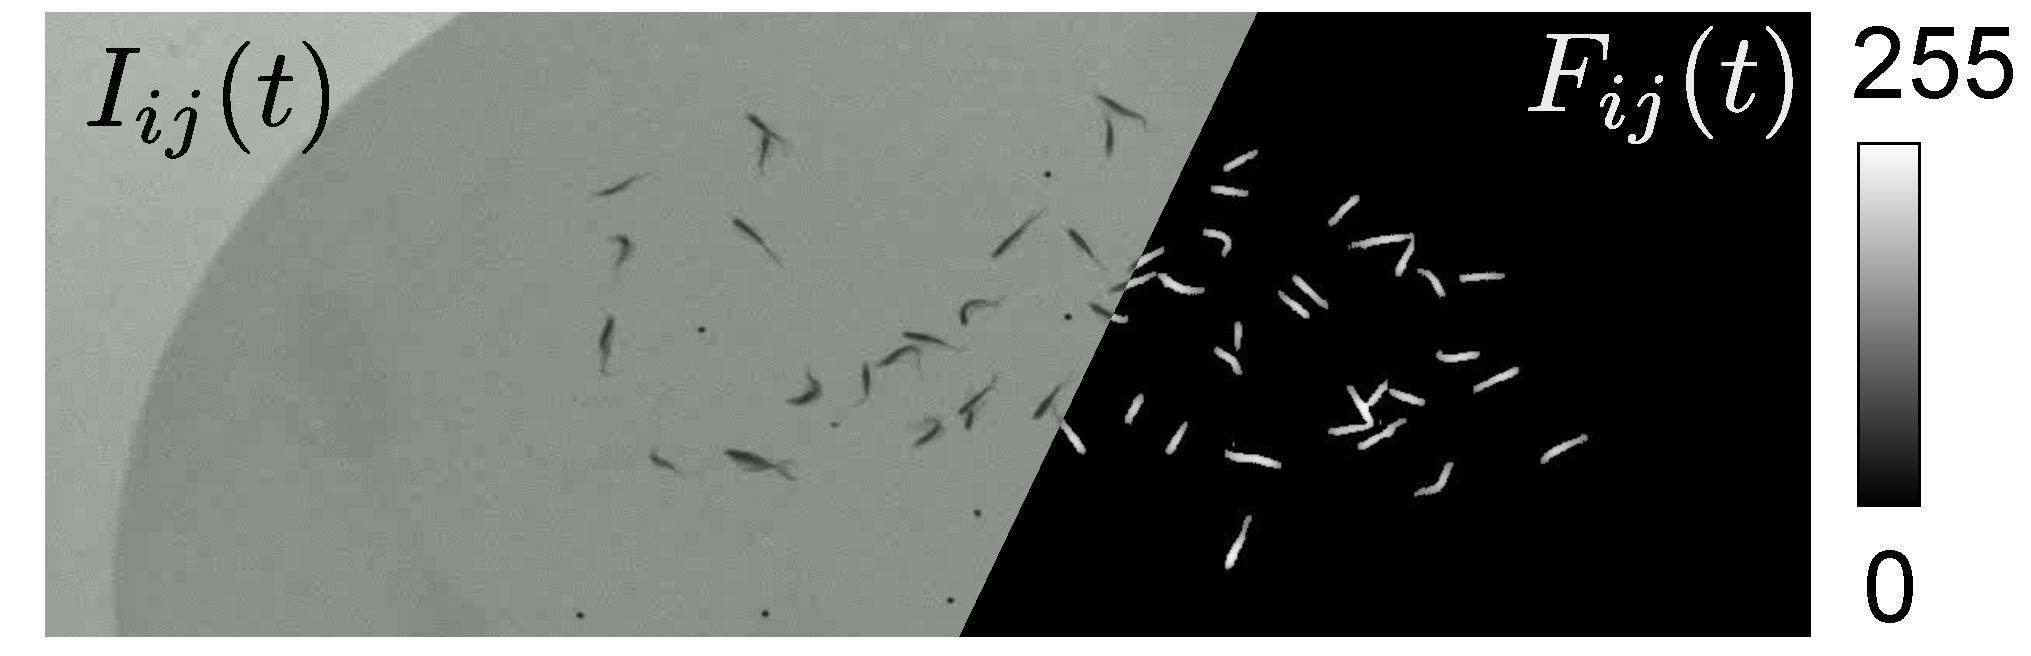
\includegraphics[width=\linewidth]{image-process}
  \caption[Two dimensional image processing.]{
  The screenshot of the video at time point $t$, and its corresponding foreground image.
  }
  \label{fig:2d_process}
\end{SCfigure}


The foreground videos of the fish are obtained after two  steps, the removal of the background and the removal of the noises. 
The background is defined as the temporal average of the image, since the fish are constantly moving while rest of the scene is static. In order to tackle the varying illumination conditions\marginfootnote{
The brightness of the environment might change in the field observation, where the sunlight might be temporally covered by the cloud. In the laboratory, the sunlight will also change the overall brightness indoors.
},
we can take a running average of a time--window, instead of calculating the overall average. The pixel intensity of the background (\gls{bijt}) at time \gls{t}, of pixel $(i, j)$, can be written as

\begin{equation}
	B_{ij}(t) = \frac{1}{T_w} \sum_{\tau=t}^{t+T}{I_{ij}(\tau)}
\label{eqBG}
\end{equation}

\noindent where \gls{iijt} is the pixel intensity of the video at time \gls{t} in position $(i, j)$, and $T_w$ is the duration of the window, usually taken as 40 seconds. The difference between the background video and original video yields a foreground video (\gls{fijt}), written as

\begin{equation}
	F_{ij}(t) = B_{ij}(t) - I_{ij}
\label{eqFG}
\end{equation}

\noindent and the order of the subtraction ensures the fish, originally appear darker in the video, to be represented by brighter pixels in the foreground video. The subtraction result can be very noisy. To remove the noise, the gaussian filter was applied to the foreground image. Then, the combination of the Ōtsu threshold and local Gaussian threshold was applied to the image, to separate the pixels belonging to the fish and other pixels.
The Ōtsu threshold is a single value that split the image into two groups, where the inter--group variance was minimised. The local Gaussian threshold, on the other hand, gives a collection of different values for different pixels, featuring the locally bright pixels as foreground. Finally, the morphological operation ``binary opening'' was applied to the image, to remove any possible remaining noise. The results shown in Fig.~\ref{fig:2d_process} was obtained with this method.

Our method requires 3 parameters, including the standard deviation (\gls{sigblur}) of the  Gaussian kernel of the blurring process, the length scale for the local threshold (\gls{llt}), and the length scale of the binary open operation (\gls{lbo}). In the different experiments, the images were similar, therefore the same set of parameters ($\sigma_\mathrm{blur}=2, l_\mathrm{local}=3, l_\mathrm{open}=3$) was applied, and works well for most videos.



\subsection{Extracting Features from the Image}
\label{section:feature}



From the processed video, we need to extract the features\marginfootnote{
We explained the term ``features'' by the end of the section.
} in each frame that correspond to the fish. In order to tackle the problem, we employed a method that not only captured the positions, but also the information of the fish orientations and body shapes. The basic idea is to calculate the cross--correlation between the image ($F_{ij}$) and a templated fish shape (\gls{tij}), as the local maxima in the result would indicate the presence of a fish, because cross--correlation is a measure of similarity between signals.


For a fixed 2D fish template (\gls{tij}), we can rotate it so that it contains $o$ different orientations. Calculating the cross-correlation of all the rotated templates, we can effectively get $o$ different results, and they can be concatenated into a 3D tensor, written as \gls{cijo}. One can think of the tensor $C_{ijo}$ as a 3D volumetric image. A local maximum in $C_{ijo}$, with coordinate $(i_m, j_m, o_m)$, indicates the presence of a fish at location $(i_m, j_m)$, with orientation $o_m$.


In addition, we are free to choose different templates for the fish shape, to capture the different postures. The choice for the template will be discussed in section~\ref{section:template}. If $s$ different shapes were selected as templates, all of which were rotated into $o$ different orientations, then there will be $s \times o$ different templates. The cross-correlation of these templates with the image would yield a 4D tensor that can be shaped into \gls{cijos}, noted as the \emph{feature tensor}. A local maximum of the feature tensor, with coordinate $(i_m, j_m, o_m, s_m)$, represents a fish located at $(i_m, j_m)$, whose shape is like the $s_m$th template, with orientation $o_m$. All the local maxima, {$\{(i_m^i, j_m^i, o_m^i, s_m^i)\}$}, captured the locations, orientations and shapes of all the fish in the image.

\begin{SCfigure}
  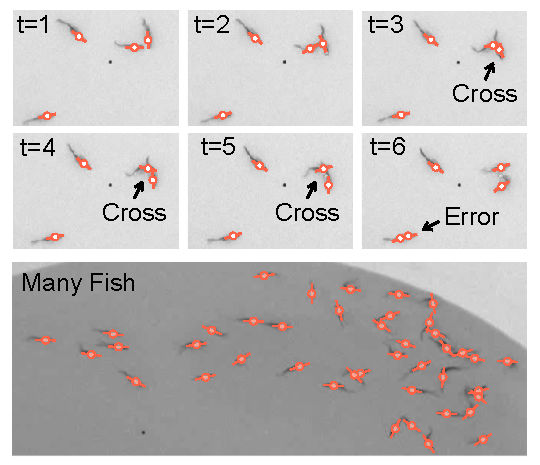
\includegraphics[width=\linewidth,outer]{features}
  \caption[The correct label of overlapping fish.]{
  The locations and orientations, $\{(i_m, j_m, o_m)\}$, of different fish. The locations are rendered as circles, while the orientations were rendered as short line segments.
  The features were calculated from the feature tensor ($C_{ijo}$).
  Top: the movement of 4 fish in 6 successive frames labelled with the detected features. An error where one fish was mistakenly labelled as two fish happened in the 6th frame.
  Bottom: the movement of many fish labelled with the detected features.
  }
  \label{fig:fish_features}
\end{SCfigure}

In summary, the cross--correlation between the image and the many templates yields a 4D feature tensor, whose local maxima give us the locations, orientations, and shapes of different fish. This approach is especially helpful for the dense system, where the fish constantly overlap with each other. In such dense scenario, the overlapping fish will be separated into different regions in the shape--rotation dimension in the feature tensor. For example, the overlapped fish pair in Fig.~\ref{fig:fish_features} was correctly labelled, by calculating the local maxima in the 4D tensor.


There is a fundamental flaw of our algorithm, where a big fish might be mistakenly labelled as two small fish. One example of such error was presented in Fig~\ref{fig:fish_features} (top row, t=6).
This is partially due to the loss of morphological details of the fish, as the cameras were placed relatively far from the fish, in order to capture larger groups.
Without the details, it can also be hard for a human being to tell, whether a dark blob is a big fish or it belongs to two smaller fish. Realistically, some of the errors produced by our algorithm can be easily distinguished by human beings. Some post processing methods of the features, based on the geometry of the fish, might be useful to further refine our algorithm. The ultimate goal is to make the feature detection algorithm being compatible with human observations.


\begin{tcolorbox}[
title={Why are features called features, not positions?},
enlarge bottom by=0.5em,
enlarge top by=0.5em,
]
In the computer vision community, people call the locations of objects ``features''. This term is rooted in the 3D reconstruction problem, which will be discussed in the chapter~\ref{chapter:fish_3d}. Briefly, the 3D information can not be recovered from the background, like a purely white wall. Instead, some ``features'' with intensity gradients are required \cite{ma2005}. Alternative names would be ``positions'' or ``locations''. However, we are interested in a ``feature'' of the photo, rather than a (physical) location of a fish.
\end{tcolorbox}

\subsection{Finding Templates for the Features}
\label{section:template}


To calculate the feature tensor $C_{ijos}$, it is important to use suitable templates for the fish. The templates should represent characteristic fish shapes.
%The unsupervised machine learning methods from the computer vision community are suitable in this situation .
The following operations were carried out to find suitable templates.

\begin{enumerate}
	\item Segment the individual fish and align the segmented images.
	\item Project all the segmented images to a space with reduced dimension.
	\item Find clusters for the data points in the reduced space, and the average of each cluster to be the template.
\end{enumerate}

The individual fish, defined as connected bright pixels, were segmented from the foreground video ($F_{ij}(t)$).
The orientation of the segmented fish were determined by the principle component analysis (\gls{PCA}) \cite{goodfellow2016}. 
These segmentations were then reoriented, so that its first principle axis align with the $x$ axis. The reoriented individual fish were then zero-padded to have the same shape, noted as $\mathbf{S} \in \mathbb{R}^{s \times s}$ where $s$ is the size of the padded images.
Examples of the segmented and aligned images are illustrated in Fig.~\ref{fig:fish_segment}. These images were collected over 1000 different frames, in a video of 4 swimming fish. A total of 3070 individual shapes were collected.

\begin{SCfigure}
  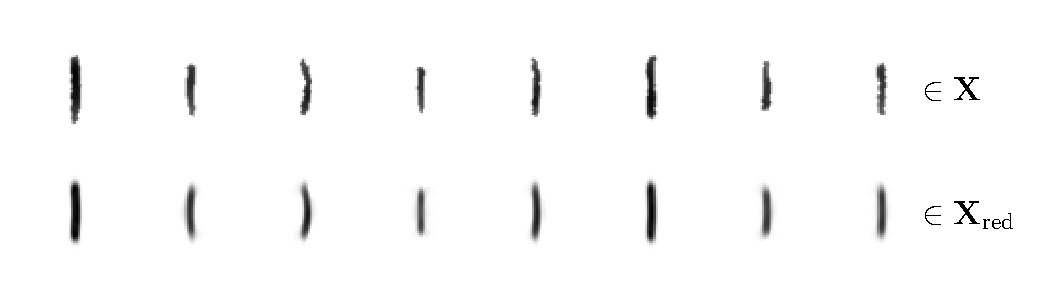
\includegraphics[width=\linewidth]{shapes}
  \caption[Examples of segmented individual fish]{
  Top: the selected individual fish segmented from the images taken by the camera.
  Bottom: the fish shapes reconstructed from a low dimensional feature space $\mathbf{X}_\mathrm{red}$.
  }
  \label{fig:fish_segment}
\end{SCfigure}

The collection of segmented fish is a very large dataset.
For example, if we use a small image of size $50 \times 50$ pixels, to stored each fish, then each fish corresponds to a point in a 2500 dimensional space.
The dimension of such images can be drastically reduced by PCA \cite{solem2012book, geron2019}. Operationally, all of the $m$ images of individual fish were flattened
($\mathbb{R}^{s \times s} \rightarrow \mathbb{R}^{s^2}$),
and concatenated into a matrix ($\mathbf{X} \in \mathbb{R}^{m \times s^2}$).% For the dataset presented in Fig.~\ref{fig:fish_segment}, $m=3070$.
The singular value decomposition (\gls{SVD}) is then performed on the dataset $\mathbf{X}$, following

$$
\mathbf{X} = \mathbf{U} \Sigma \mathbf{V}^T,
$$

\noindent where the matrices $\mathbf{U}$ and $\mathbf{V}$ contains all the left and right singular vectors, and the matrix $\Sigma$ contains all the singular values. The images ($\mathbf{X}$) were then project on the first $k$ axes ordered by their corresponding singular values. Effectively, the dimension of the matrix $\mathbf{X}$ were reduced from $m \times s^2$ to $m \times k$, forming a new matrix $\mathbf{X}_\text{red} \in \mathbb{R}^{m \times k}$. Each row in $\mathbf{X}_\text{red}$ described one fish.



Figure~\ref{fig:fish_pca} shows the average fish shape as well as the projection of all the segmented fish ($\mathbf{X}$) on the first two principle axes. The first principle axis (the $x$ axis of Fig.~\ref{fig:fish_pca}) roughly captured the scale of the fish, and the second principle axis (the $y$ axis of Fig.~\ref{fig:fish_pca}) captures the information about the bending of the fish. 
The overall distribution of those projected data can be understood by the fact that the same fish can have different distances and orientations, relative to the camera, so that their shapes will appear different.
The distribution of Fig.~\ref{fig:fish_pca} is symmetric in the $y$ direction, which indicates the absence of chirality for the bending of fish. That is to say, the fish do not prefer bending to the left, or the right.

With all the segmented fish being projected to low dimensional space, we can use the \emph{k-means cluster} algorithm to find representative cliques of the fish shapes.
Briefly, different data points (different fish images in Fig.~\ref{fig:fish_segment}) will be assigned to different clusters. And the variance of points in the same cluster will be minimised, while the variance of points from different clusters will be maximised.

Each cluster corresponds to similar fish images with similar shapes. The average shape of different clusters were used as the template. The different scatters in Fig.~\ref{fig:fish_pca} shows the different clusters, and their corresponding average shapers were inserted. Here, the images ($\mathbf{X}$) were projected to a 2 dimensional space ($k = 2, \mathbf{X}_\text{red} \in \mathbb{R}^{3070 \times 2}$). And the overall 3070 points were separated into 7 different clusters. And the average shape of different clusters (the inserted subplots in Fig.~\ref{fig:fish_pca}) can be used as the templates to calculate the 4D tensor for tracking.



\begin{SCfigure}
  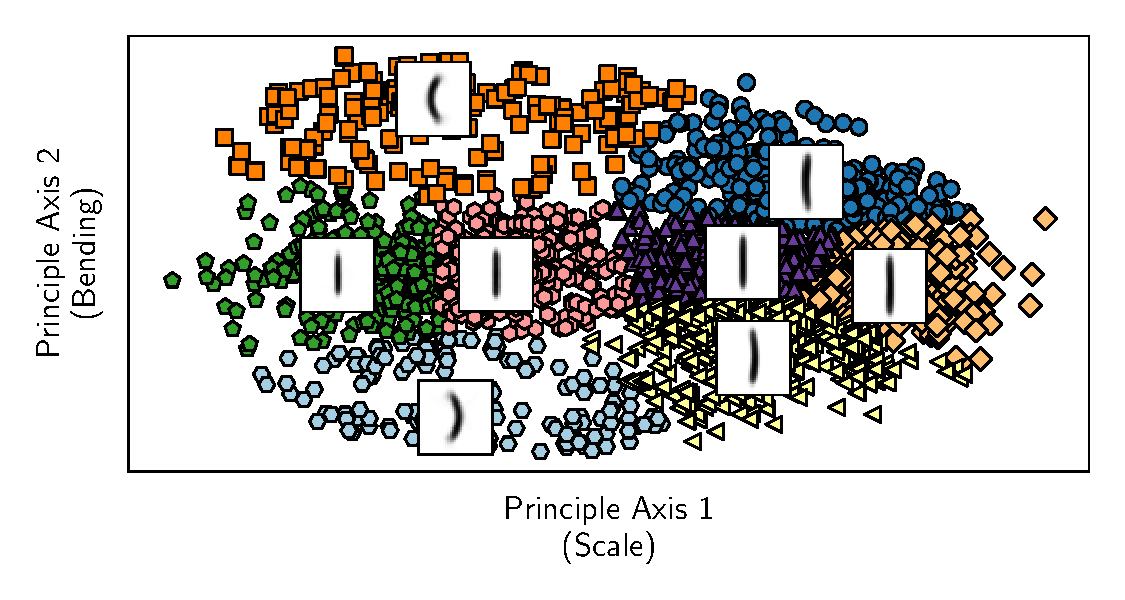
\includegraphics[width=\linewidth]{fish-pca-proj}
  \caption[PCA analysis of the fish shape]{
  A collection of 2170 different fish shapes, projected onto the first two principle component axes. The data points were clustered using the K-means algorithm, into six different clusters, indicated by different marker styles. The average shape of each cluster were plotted in the inserted axes.
  }
  \label{fig:fish_pca}
\end{SCfigure}


The number of clusters and the dimension of the reduced space ($k$) are free parameters, whose optimal values were hard to determine. Practically, I always set $k=5$, and separate the points into 8 different clusters, which yields good\marginfootnote{
If the 2D features are not good, the corresponding 3D reconstruction (chapter~\ref{chapter:fish_3d}) will fail.
} results for 2D tracking. The dimensional reduction method (PCA) and the clustering algorithm (K-means) can be changed to other tools with similar effects. For instance, it is possible to use non-linear dimensional reduction method such as isomap, and a gaussian mixture model to obtain different clusters.

The mapping from the image to the large 4D tensor, $I_{ij} \rightarrow C_{ijos}$ requires a large amount of calculation. The feature tensor is normally sparse, since only a few pixels in the image contain the centre of the fish. The calculation can be faster if such sparsity were to be exploited.
Practically, we can only calculate ``promising'' pixels, where fish is likely to appear. These pixels correspond to the local intensity maxima in the foreground image $F_{ij}$. Such reduction of calculation improved the calculation speed significantly.


\subsection{Convolutional Neural Network}
\label{section:cnn}



There are two steps in the image processing that can be improved in the image processing pipeline. The first one is the removal of background. In my current method, I calculated a rolling average of the entire video. The window size of the averaging operation is set by the user, which is very difficult to optimise because the video processing typically takes hours to finish. Practically, a rule-of-thumb number (600 frames) was applied. However, the fish in the video are very distinct from their background, and it is an easy task for people to spot the fish in a static image. This suggests a static image contains enough information to distinguish the foreground (fish) and background (tank). 

The convolutional neural network (\gls{CNN}) is very suitable for carrying out both tasks at the same time, with far better efficiency. The overall data process introduced from section~\ref{section:image_process} to section~\ref{section:template}, is essentially a transformation from the image ($I_{ij}$) to a tensor ($C_{ijos}$). In addition, the information about the kernel is unnecessary\marginfootnote{
The shapes might be informative for people studying the postures of the swimming fish. But we will ignore the shapes in this thesis as we are interested in the \emph{collective motion} of the fish.
} in most cases, as we often only care about the orientation and location of the fish, rather than its shape. Hence, we need a model with the capacity to carryout the following transformations depending on our desired results:

$$
\begin{aligned}
I_{ij} &\rightarrow C_{ijos} 
&\textrm{location, orientation, and shape} \\[1ex]
I_{ij} &\rightarrow C_{ijo}\;(= \max_{s}{C_{ijos}})
&\textrm{location, and orientation} \\
I_{ij} &\rightarrow C_{ij}\;(= \max_{o}{C_{ijo}})
& \textrm{location} \\
\end{aligned}
$$

\noindent And we can generate a big dataset containing images ($I_{ij}$) and their corresponding feature tensors ($C_{ijos}$), and make a CNN to learn the underlying rules for the transformation ($I_{ij} \rightarrow C_{ijos}$). If we need less information from the result, the targeted $C$ can be contracted, by taking the maximum value along the dimension of the unnecessary information.

\begin{SCfigure}
  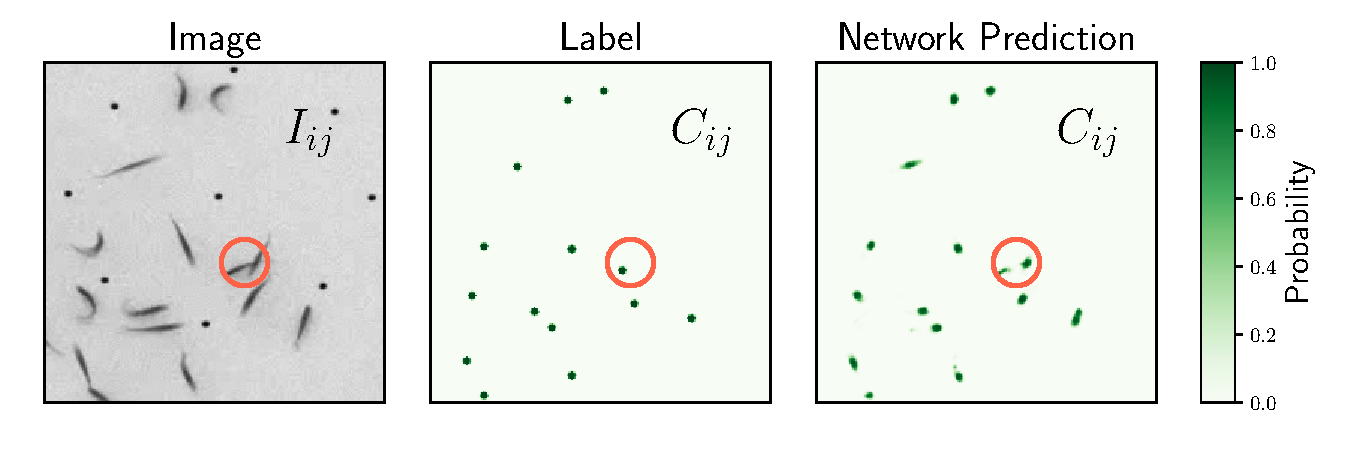
\includegraphics[width=\linewidth]{locate-cnn}
  \caption[The feature tensor calculated with convolutional neural network]{
	The tracking result of a convolutional neural network (CNN).
	Left: the image ($I_{ij}$) from which the fish will be detected. (The black dots in the image are the holes drilled on the tank.)
	Middle: the feature tensor (\gls{cij}) for all the pixels generated by a conventional 2D tracking algorithm. This data is used as training data for the neural network. The value of a pixel in the tensor represents the probability that a fish centre being located inside this pixel. 
	Right: the feature tensor ($C_{ij}$) for all the pixels predicted by the CNN model. The network prediction should be close to the label after the network being trained.
  }
  \label{fig:locate-cnn}
\end{SCfigure}


As a proof of concept, a CNN model was built to carry out the transformation of $I_{ij} \rightarrow C_{ij}$. The training data for the network was generated from the existing tracking result $C_{ijos}$.
The model was built with popular framework tensorflow \cite{tensorflow2015}, and trained on the Colab online platform provided by Google \cite{carneiro2018}.
Figure~\ref{fig:locate-cnn} shows the output of a trained network. The network does not generate the exact same picture of the label, but their results were similar. Notably, the network even fixed an error of the original feature detection algorithm. This error is highlighted in Fig.~\ref{fig:locate-cnn}. 

However, due to the limited time for this project, the final CNN model did not improve the calculation accuracy nor the processing speed significantly. Nevertheless, it is achievable to having the calculations to be optimised that the tracking can be performed in real time, since the prediction of $C_{ij}$ on a GPU is very fast, reaching a speed of $\sim 50$ frames per second. The current speed-limiting step is the calculation of local maxima in $C_{ij}$ with CPU. This calculation can be accelerated by either exploiting the sparsity of $C_{ij}$, where local maxima detection can be converted to an overlapping removing problem (see section \ref{section:overlap}). Alternatively, it might also be helpful to carry out the calculation on GPU.


\section{Results}

In this section, the spatial distribution of zebrafish will be presented. For all the data shown below, the fish that were not swimming was excluded from the calculation. The swimming fish was defined as the fish whose swimming speed is larger than 60 mm/s. This specific value was chosen, based on the fact that the average speed of zebrafish is around 120 mm/s.

\subsection{A Single Fish}
\label{section:fish_1_2d}

\marginpar{
\centering
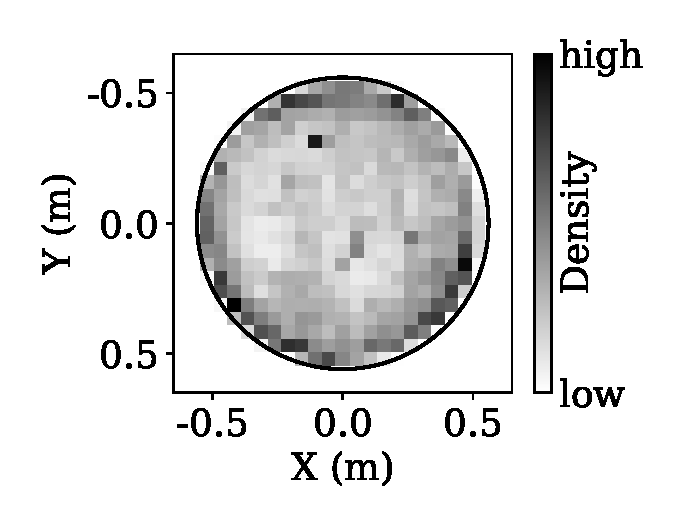
\includegraphics[width=\marginparwidth]{dist-1-fish}
\captionof{figure}[The 2D spatial distribution of 1 adult zebrafish]{
The spatial distribution of one adult zebrafish in a quasi 2D environment, present the joint distribution of the $x$ coordinates and $y$ coordinates of the fish positions, with the shape of the boundary being highlighted.
}
\label{fig:density_2d_fish_1}
}


Figure~\ref{fig:density_2d_fish_1} shows the spatial distribution of one adult wildtype zebrafish. We can see from the figure that the fish have a slightly higher tendency to stay near the boundary. The apparent attraction between the fish and the boundary can have two reasons. Firstly, the fish may biologically prefer to be near the boundary. The systematic preference for the wall of the tank was documented for zebrafish previously \cite{seguret2016}. 

In addition, the preference to the wall of the fish could emerge as a physical consequence, if we think of fish as self-propelling particles \cite{lee2013, maggi2015, bechinger2016}, as justified in section~\ref{section:active-matter}. To understand this physical origin, it is helpful to to imagine a fish who changes its orientation randomly. Without the boundary, the fish would move constantly, regardless of its orientation. On the other hand, if the fish were swimming against the wall, they have to wait until the orientation changes, to leave the wall and continue swimming. The extra waiting period near the wall would contribute to the spatial distribution.



\subsection{Two Fish}
\label{section:fish_2_2d}

The movement of 2 adult zebrafish was recorded. The data was taken over 5 experiments, and each experiment lasted one hour.
The spatial distribution of 2 fish were shown in Fig.~\ref{fig:density_2d_fish_2} (left). It is clear that the fish were not uniformly distributed in the tank, which might also related to the environmental factors, such as the illumination level \cite{makris2006, rosemberg2011, shelton2020}. Practically, we also found the zebrafish would respond to the shadows casted by the objects around the tank.

\begin{SCfigure}[][!ht]
  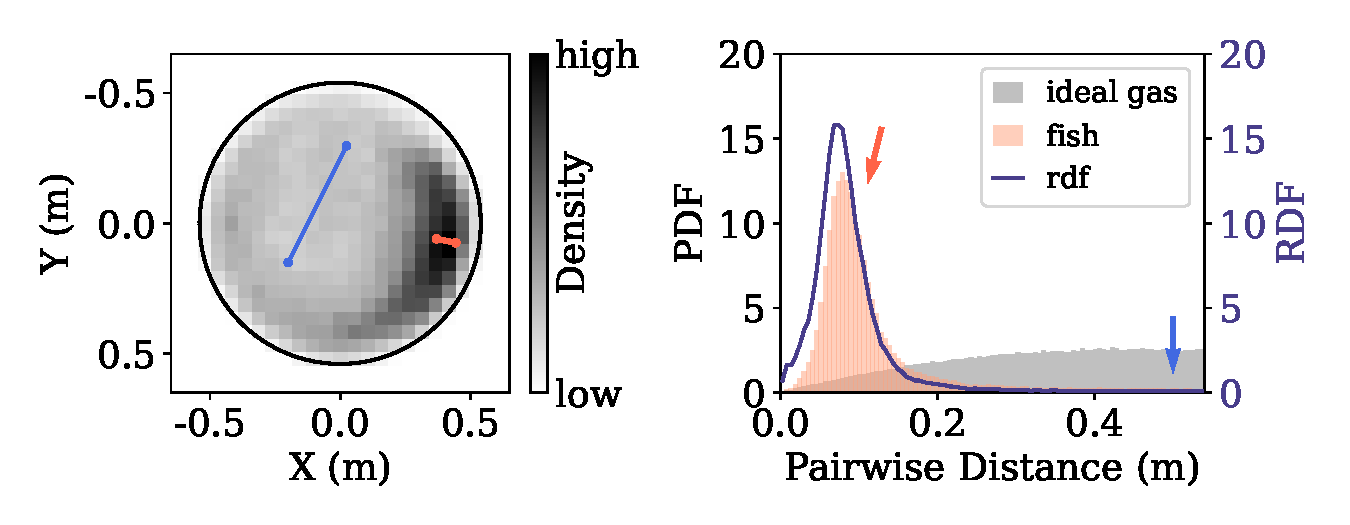
\includegraphics[width=\linewidth]{dist-2-fish}
  \caption[The 2D spatial distribution of two fish]{The spatial distribution of two adult zebrafish in a quasi 2D environment. Left: the joint distribution of the $X$ coordinates and $Y$ coordinates of the fish positions, with the shape of the boundary being highlighted.
  Right: the probability density function (PDF) for the distance between two fish. The PDF for the distance of 2 ideal gas particles, uniformly distributed in the tank, were also plotted. The ratio of the two \gls{PDF}s were taken as the radial distribution function (RDF).}
  \label{fig:density_2d_fish_2}
\end{SCfigure}

The pairwise distance of the 2 fish offered us the way the characterise their cohesion. If the fish were attracted to each other, they would stay close, and vice versa. The distribution of the pairwise distances, shown as the probability density function (PDF), were plotted in the Fig.~\ref{fig:density_2d_fish_2} (right). There is a peak in the distribution, and it seems to be dominated by the inhomogeneous distribution of the fish, as the length scale corresponding to the peak matches the size of the high density blob. Such a length scale was highlighted in Fig.~\ref{fig:density_2d_fish_2} (left).




It is useful to compare the distribution of the pairwise distance of the fish, with the distribution from the ideal gas. Here ideal gas means random points uniformly distributed in the circular tank outlined in Fig.~\ref{fig:density_2d_fish_2}. The distribution of the ideal gas were presented in Fig.~\ref{fig:density_2d_fish_2} (right). The probability of finding particles at large distances, like 0.5 meter, is higher for the ideal gas particles comparing with fish. This is also likely due to the inhomogeneous distribution of the fish, as such length scale corresponds to a big ``void'' in Fig.~\ref{fig:density_2d_fish_2}.

Inspired by liquid state theory, we define the ratio between the PDF of the fish and that of the ideal gas as the radial distribution function (\gls{RDF}), which is also known as the \gls{gr}, as introduced in section~\ref{section:intro-analysis}.
For a dilute fluid at equilibrium, the shape of its RDF can be used to calculate the pairwise interaction potential. The mapping between pairwise potential and the $g(r)$ is invalid for the fish, because the individuals were constantly spending their biological energy to swim, driving the system out of equilibrium.
Nevertheless, $g(r)$ is still a useful tool to characterise the cohesiveness of the fish group. The RDF of 2 fish are plotted in Fig.~\ref{fig:density_2d_fish_2}, and it presents a peak at very short separation. The hight of the peak ($\sim 15$) offered a measure of the attraction amongst the fish, and more detailed analysis will be provided in chapter~\ref{chapter:fish_analysis}.


\subsection{Three Fish}
\label{section:fish_3_2d}


\begin{SCfigure}
  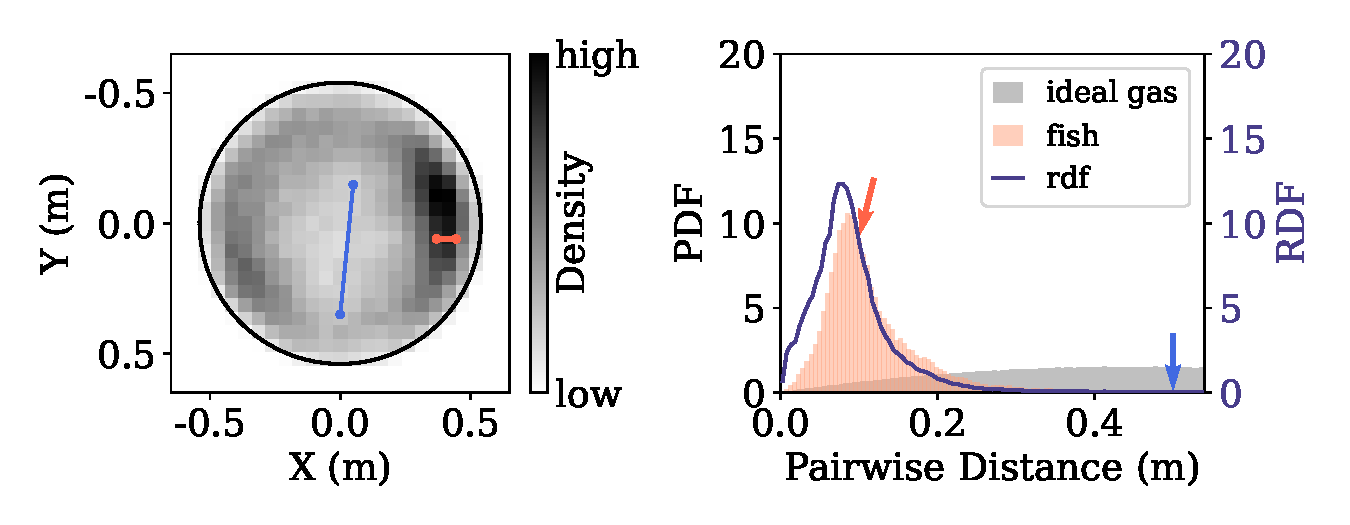
\includegraphics[width=\linewidth]{dist-3-fish}
  \caption[The 2D spatial distribution of three fish]{The spatial distribution of three adult zebrafish in a quasi 2D environment. Left: the joint distribution of the $X$ coordinates and $Y$ coordinates of the fish positions, with the shape of the boundary being highlighted. Right: the probability density function (PDF) for the distance between two fish. The PDF for the distance of 3 ideal gas, uniformly distributed in the tank, were also plotted. The ratio of the two PDFs were taken as the radial distribution function (RDF).}
  \label{fig:density_2d_fish_3}
\end{SCfigure}


The behaviour of 3 adult zebrafish is very similar to that from 2 fish. The density distribution and the distribution of pairwise distances of 3 zebrafish were shown in Fig.~\ref{fig:density_2d_fish_3}. Like the situations in the one fish and 2 fish system, the distribution is not uniform. And the fish also present a typical peak in the pairwise distance, whose location (~0.08 m) corresponds to the size of the high density blob of the inhomogeneous distribution.


Comparing the PDF of the pairwise distance of the fish, with that from 3 ideal gas, the fish also presents the typical void like the 2 fish scenario. The RDF for 3 fish, shown in Fig.~\ref{fig:density_2d_fish_3} (right) is very similar to that of 2 fish. The height value of the peak for 3 fish is close to 12, being slightly smaller than that from 2 fish experiments. One possible explanation for such reduced attraction, is the reduced danger perceived by the fish, when they were in a large group \cite{spence2007}.
%\marginfootnote{This reference is not very convincing.}.
As the fish will form a denser group when they perceived danger \cite{perez-escudero2017}.
 As well be presented later, the reduced cohesion with increased group number is a general observation.



\subsection{Many Fish}
\label{section:fish_50_2d}

The distribution of 50 fish was significantly different from the 1/2/3 fish results, as presented in Fig.~\ref{fig:density_2d_fish_50}.
Comparing with the 1/2/3 fish experimental results, the density distribution of 50 fish were more homogeneous, shown in the left subfigure in Fig.~\ref{fig:density_2d_fish_50}. However, it is still not uniform. The homogenised picture for 50 fish might be related to the fact, that the fish-fish interaction dominates the behaviour for 50 fish, while fish-environment interaction dominates the behaviour of 1/2/3 fish. The same trend was also observed in a 3D swimming experiment, which will be discussed in section~\ref{section:fish_many_3d}.

In addition, the PDF of the pairwise distance for 50 fish were much broader comparing with its 2 or 3 fish counterpart. Nevertheless, we still see the same trend, where the fish were cohesive in short length scales, and presented ``void'' at larger separation distances. Such feature is also likely due to the inhomogeneity of the density distribution. However, the difference of the PDFs for the 50 fish and 50 ideal gas particles was less significant. As a result, the RDF of the 50 fish contains only a broad peak, whose height value ($\sim$ 3) is significantly smaller the height value of the RDF for 2 or 3 fish. This suggested a smaller effective attraction\marginfootnote{
The ``attraction'' is unlikely to be biased by our choice of the measurement, the RDF. The RDF is effectively a re-weighted PDF of the pairwise distances. Other measurements of the fish-fish distances are therefore related to the RDF in different ways, which will be discussed in Chapter~\ref{chapter:fish_analysis}. As an example, the nearest neighbour distance is proportional to the height of the peak in the RDF (Fig.~\ref{fig:change-states-2d} and \ref{fig:change-states-3d} in Ch.~\ref{chapter:fish_analysis}).
} between the fish when they were in a large group. Our observation, the reduction of peak height in the RDF, is consistent with previous study \cite{romenskyy2017}.

\begin{SCfigure}
  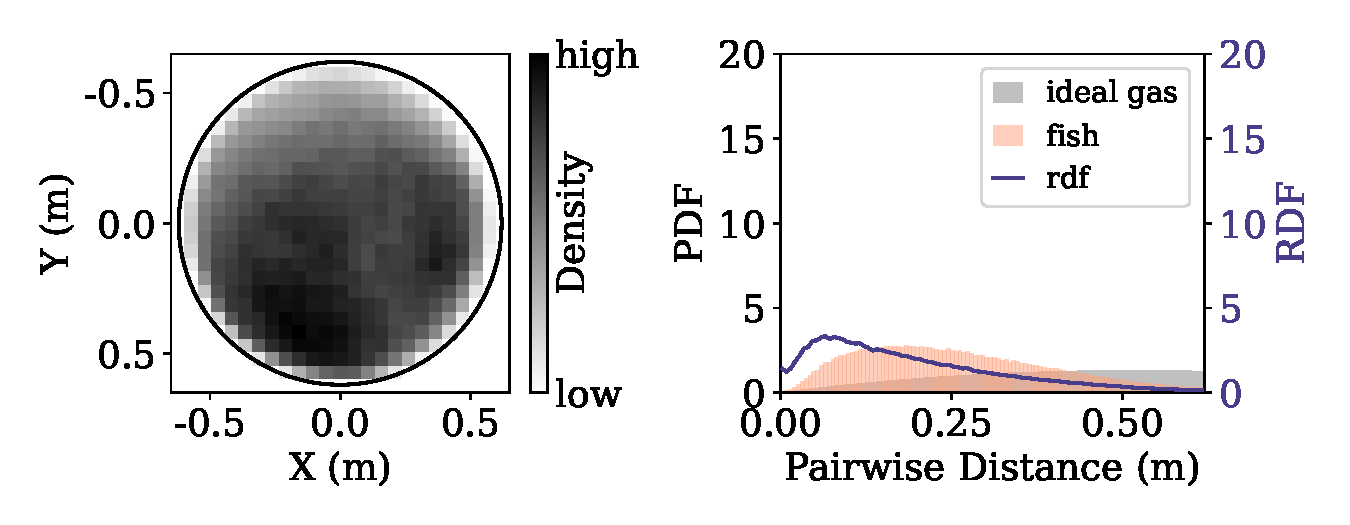
\includegraphics[width=\linewidth]{dist-50-fish}
  \caption[The 2D spatial distribution of 50 fish]{The spatial distribution of 50 adult zebrafish in a quasi 2D environment. Left: the joint distribution of the $X$ coordinates and $Y$ coordinates of the fish positions, with the shape of the boundary being highlighted. Right: the probability density function (PDF) for the distance between two fish. The PDF for the distance of 50 ideal gas particles, uniformly distributed in the tank, were also plotted. The ratio of the two PDFs were taken as the radial distribution function (RDF).}
  \label{fig:density_2d_fish_50}
\end{SCfigure}

\vfill
\pagebreak


\begin{adjustwidth}{0cm}{-5cm}
\begin{tcolorbox}[
fonttitle=\sffamily\Large,
right=0.1\linewidth,
top=5mm,
bottom=5mm,
title=Summary of Chapter~3,
]

\begin{itemize}
	\item Locating a group of fish in 2D is necessary for their 3D reconstruction. For this task, existing methods utilise the morphological details of the fish for identification. These methods are only accurate for fish swimming in a quasi-2D system.
	\item We proposed a new method to locate fish in 2D, where the fish are swimming in a 3D environment. Our method includes the following process.
	\begin{description}
		\item[0. Metric Rectification (optional)] \hfill \\ 
		The distortion and imperfect orientation can be removed by camera calibration.
		\item[1. Image Processing] \hfill \\ 
		The images, captured by the cameras, are separated into the foreground and the background.
		\item[2. Finding Templates] \hfill \\ 
		The individual fish in the foreground are segmented, aligned, and projected to a low dimensional space. Characteristic shapes were identified with clustering algorithm for data points in the low dimensional space.
		\item[3. Constructing the Feature Tensor] \hfill \\ 
		The templates were rotated into different orientations. For every template and orientation, its cross-correlation with the foreground is calculated. The results correspond to a 4D feature tensor.
		\item[4. Extracting the Features] \hfill \\ 
		Local maxima in the 4D feature tensor correspond to the locations, orientations, and shapes of the fish in the image. Each maximum is called a feature in the image.
	\end{description}
	\item We reported the analysis on the coordinates of zebrafish in a quasi-2D environment, featuring different fish numbers.
	\begin{description}
		\item[One Fish] \hfill \\
		The fish tend to swim near the boundary.
		\item[Two Fish] \hfill \\
		The fish tend to swim near one side of the boundary. The heterogeneity of the spatial distribution dominated the radial distribution function.
		\item[Three Fish] \hfill \\
		The behaviour of three adult zebrafish is very similar to that from two fish.
		\item[Fifty Fish] \hfill \\
		The spatial distribution of 50 fish presented a more uniformed manner, with significantly reduced cohesiveness.
	\end{description}
\end{itemize}
\end{tcolorbox}

\end{adjustwidth}

\end{document}